\chapter{Inter-Process Communication}
\label{sec:interProcessCommunication}

Inter-process communication (IPC) is the way that any two processes communicate with each other.  This can include processes in different applications, such as a web server sending webpages to a web browser, or separate processes of the same application, such as \texttt{Spotify} and \texttt{Spotify Helper} working together to play music.  When this communication occurs within one computer, it is local IPC.


\section{Benefits of IPC}
\label{sec:benefitsOfIPC}
There are many situations that are well-solved by having a multi-process application.  These are normally problems that have multiple distinct functions, since each task can be separated into its own process.  Examples of applications that fall into this category include web servers, password managers, and \texttt{XWindows}.

\subsection{Web Servers}
\label{sec:webServers}
Web servers have the difficult job of serving thousands, if not millions, of connections at the same time.  One method to deal with this is to use multiple processes, one for each of the new connections, and one parent process to accept new ones.  The parent process starts listening on the desired port, and accepts every new connection that is made.  Then, it creates a new process which is in charge of servicing a single connection.  In this structure, each child concerns itself with only one client, and can serve data and webpages as fast as it can be scheduled.  The parent is then left alone to accept connections without needing to worry about individual clients.

By keeping the tasks of accepting and servicing connections independent of each other, a web server can work more efficiently.  If one process had to do both jobs, then it would accept a connection and service it until the client disconnected, and only then be able to accept a second connection.  This means that only one connection would be allowed at a time, an unacceptable condition for a web server.  Therefore, there needs to be some form of parallelism so that new connections can be accepted while also satisfying already connected clients.  In this case, new processes create this paralellism, but a similar solution spins off a new thread for each connection.  Both of these systems allow web servers to provide immense amounts of data to clients, much more than would be possible by a single, single-threaded process.

\subsection{Password Managers}
\label{sec:passwordManagers}
\subsubsection{Password Manager Usage}
\label{sec:passwordManagerUsage}
Password managers also make use of multiple processes to separate the different jobs they perform.  Password managers are used to help make a user's passwords more secure.  It is difficult for users to come up with strong passwords since the recommendations for a good password---long, random assortments of letters, numbers and special characters---are the same strings that are extremely hard for humans to memorize.  It is impossible for users to memorize a unique, strong password for every single account they have.  Instead, users will often choose weak passwords and repeat them over many accounts, since this lowers their cognitive burden.  Password managers strive to make passwords more secure by remembering all but one of a user's passwords.  All the user needs to know is the one master password to unlock the manager.  Then, the user will be able to either read, copy or autofill the password from the manager and into the application.

A password manager often has two separate ways to help users; it can display the passwords to the user or autofill them into a form.  To display the passwords, the manager will have an application designed to let users easily view and change their saved passwords.  The application will open, and the user will be prompted to enter his or her master password.  This will unlock the password vault, which is the process in the background that holds the passwords and sends them when a valid request is made.  Once the vault is unlocked, the user will be presented with the different account names that are saved---a Google account, a banking account, and an ESPN.com account---for example.  Once a user clicks on the desired account, the password will be fetched from the vault and shown to the user.  There may also be a feature that would allow the user to copy the password, so as to paste it into a form later.  When the user closes the application, the vault will be locked again.

The other way that password managers are often used is to autofill usernames and passwords into web browsers.  They do this by using a browser extension.  For example, when you download \texttt{1Password}, you are able to download the desktop application and the browser extension.  When using a browser extension, if the user travels to a webpage that has sign-on information, GMail for example, either the user will be able to choose the username and password saved in their password manager for their GMail account or the password manager will guess the desired credentials and autofill them for the user.  This way, users can easily enter their passwords on websites without ever having to leave their web browser.

\subsubsection{Password Manager Processes}
\label{sec:passwordManagerProcesses}
Because of the different jobs that password managers must accomplish, they are an ideal candidate to split the tasks into multiple processes.  A password manager may have three processes running at one time.  One process is the vault, which encrypts and secures the passwords on disk, ensuring that no malicious user can access the plaintext of the passwords.  Some of these vaults go so far as to create fake sets of passwords, so that an attacker would not know which set of encrypted passwords is real~\cite{bojinov2010kamouflage}.  A second running process is the desktop application to let a user read or edit their passwords, and a third process would be a browser extension to autofill passwords into webpages.  These last two processes need to communicate with the vault process so that they can receive the passwords.  The browser extension needs the plaintext of the password before it can put it into the webform, as does the desktop app before it can display the password to the user.  The communication occurs via local IPC, since all three processes would run on a single host.

Password managers lend themselves to having multiple processes because all three processes solve different jobs.  The password vault needs to keep the passwords encrypted and secure from outside access, but needs to provide the password when either of the other two processes legitimately requests it.  The desktop app should provide an easy-to-use user interface so that the user can edit or view the desired password.  Finally, the browser extension needs to find password fields in online forms and automatically fill them with the correct password based on the URL of the webpage.  By splitting each task into its own process, each can be optimized for its use.  As long as the passwords can be communicated between the processes, they will be able to work together and function as a successful password manager.

\subsection{\texttt{XWindows}}
\label{sec:xwindows}
\texttt{XWindows} is another application that benefits from using multiple processes.  \texttt{XWindows} is a program that displays graphics on a monitor.  It uses many processes, often multiple clients and one server, to create and present the images.  The server process takes in input from the mouse, keyboard, and other peripherals and sends it to the correct client, while also receiving information from the clients about what should be displayed~\cite{Scheifler:1986:XWS:22949.24053}.  Each client process is a different application which takes in mouse and keyboard data, does computation using this and the current state of the application and sends to the server what it would like to be shown on the screen~\cite{Scheifler:1986:XWS:22949.24053}.  Using this model, one server can have many clients connected to it.  This allows a single screen to display multiple applications at the same time, since each application has its own client.  Also, this means that the server can demultiplex incoming signals from the mouse and keyboard and send them to the correct client.  This architecture also allows a single application to be displayed on multiple screens, since a client can connect to multiple servers.  \texttt{XWindows} would almost certainly be unable to achieve the same benefits if it was a single-process application.  The benefits gained from using multiple processes cannot be replicated with a single process.

In early uses of \texttt{XWindows}, the client computation would be done on a separate machine from where the monitor and peripherals were located.  This allowed the machine the user interacted with to quickly demultiplex inputs from the user to the clients and multiplex the images from each client to the monitor.  This would be done using a networked connection.  Now, computer processors have enough power that these tasks do not need to be split onto separate computers, but can be accomplished on a single host.  In this case, \texttt{XWindows} will no longer use the Internet to communicate, but instead will use local inter-process communication~\cite[p 373]{Stevens:1997:UNP:522800}.

\section{Background}
\label{sec:localIPCBackground}
Local IPC is inter-process communication that occurs entirely within a single computer.  Both password managers and \texttt{XWindows}, described above, utilize local IPC often.  Many password managers exist completely within one computer, so they only communicate the passwords within that host.  The \texttt{XWindows} clients and server are often run within a computer as well.  In these scenarios, they use local IPC to efficiently communicate and work together.  Local IPC has the benefit of avoiding some of the overhead required for networked communication since it is guaranteed to stay within the computer.  This can make local IPC significantly faster than networked communication.  The tradeoffs of using different forms of local IPC will be discussed further in Section~\ref{sec:localIPCTradeoffs}.

With networked communication, the messages go through other people's computers, making the communication intrinsically insecure.  However, since local IPC never leaves the host, the security implications of the communication are less clear.  Some security experts believe that it is pointless to defend against local attackers, the same type of attackers who perform Man-in-the-Machine attacks~\cite{MitMa}.  However, if software developers used the same best practices for key-exchange protocols, encryption, and two-way authentication that are used in networked communication, then there would be no difference between the attacks possible on networked and local IPC.  Unfortunately, software has often been written without these standards extended to local IPC, creating the possibility for Man-in-the-Machine attacks.

\section{Forms of Local IPC}
\label{sec:formsOfLocalIPC}
This thesis studies three forms of local IPC: communication through Internet-domain sockets on the loopback interface, UNIX domain sockets, and named pipes.  I will discuss each in more detail here.

\subsection{Internet-Domain Sockets via Localhost}
\label{sec:localhost}
\textit{localhost} is the name traditionally associated with the IP address assigned to the loopback interface: 127.0.0.1.  Computers often provide the loopback interface as a way to communicate within themselves, using the complete network stack, without the messages leaving the machine.  It is especially useful when testing networked applications without a working Internet connection.  However, this interface is also used for local inter-process communication.  One of the benefits of using localhost for local IPC is that the entire infrastructure used for networked communication can stay the same.  The only change that needs to be made is to use the IP address of the loopback interface instead of the IP address of another, possibly remote, interface.

When communicating over localhost, a message is sent using the entire network protocol stack, including the link, network, and transport layers.  Each layer contains a header, which provides metadata about that layer, and data, which can be any assortment of bits.  For example, IP is a protocol in the network layer, so it sits in between the link and transport layers.  An IP packet has a header that contains the source and destination IP addresses, a checksum, and a field that describes the type of information contained in the data section.  Then, in the data section, an entire TCP or UDP packet would be contained, which would hold the TCP or UDP header, as well as the data inside of that layer.  This process is called encapsulation, since each higher layer is encapsulated as data within the next outer layer, and is shown in Figure~\ref{fig:encapsulation}.

\begin{figure}
\centering
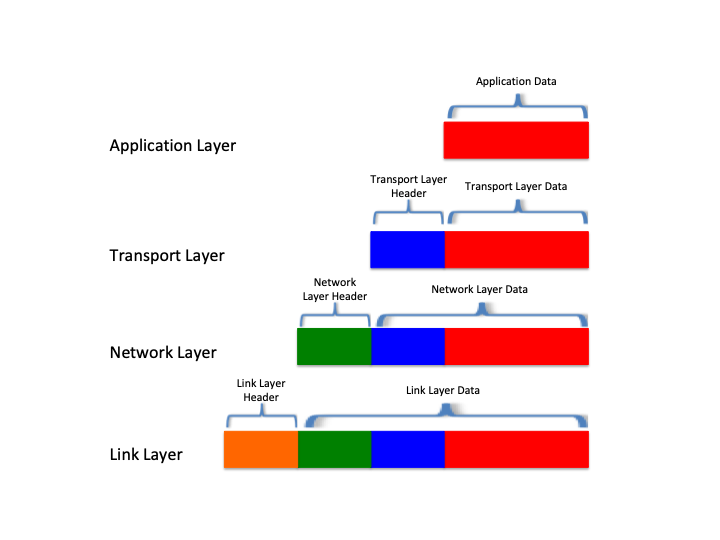
\includegraphics[width=0.75\textwidth]{encapsulation.png}
\caption{Internet Socket Encapsulation}
\label{fig:encapsulation}
\end{figure}

The link layer is used to differentiate which computer on a physical wire should accept incoming frames.  A normal Ethernet frame contains the source and destination MAC addresses, each six bytes long, as well as two bytes to indicate the network layer being used.  However, when using localhost, this can be optimized, since only one computer, the current host, is on the ``wire'' and it should listen to all incoming connections to localhost.  Therefore, when using localhost, the entire link layer header is only a four byte field that determines the family of network layer.  Most of the time, this will be IP, which has been assigned the value \texttt{2}.

The network layer used when communicating over localhost is the same as is used for networked IPC; this layer is predominantly IP.  The IP header contains information about what interface the packet is destined for, as well as what type of data is contained inside~\cite{RFC0791}.  While the Ethernet layer can be condensed when communicating through the loopback interface, the IP layer cannot, because the kernel needs to know what interface to send the packet to, which is represented in this layer.  The kernel has to route the packet to the code to encapsulate the IP packet as either an Ethernet or localhost frame, so must be able to know the destination IP address.

The next layer commonly used in the network protocol stack is the transport layer.  This layer contains port numbers to identify the source and destination processes.  The common transport layer protocols are TCP, which sends a stream of data, and UDP, which sends individual frames, called datagrams.  TCP also adds a guarantee of delivery and in-order delivery using sequence numbers~\cite{RFC0793} which UDP and the network layer protocols do not have.  Like the network layer, this layer is needed because the kernel needs to know which process to give the packet to.

Inside of the transport layer is the application layer.  This can be a popular protocol like HTTP or the ``BitTorrent'' protocol, or it can be a proprietary protocol.  Many applications have their own application layer protocol to transmit the exact information that is needed in a precise format.  Encryption and other forms of security are also added at this layer.

When a process uses the loopback interface to communicate with another process, it uses this entire protocol stack: the condensed link layer, the network layer, the transport layer, and the application layer.  This makes localhost very useful for a programmer, since from a programming perspective, the code is the exact same as the code for networked communication, except for the destination IP address.  There is no need to use different data structures or macro values, since the communication almost completely mocks real Internet communication.  Also, if there is a possibility that the communication endpoint will change to a remote interface, it is very easy to modify the code since only the destination IP address would be changed.

Code samples of a TCP server and client are given in Appendices~\ref{appendix:loopbackTcpServer} and~\ref{appendix:loopbackTcpClient}.  A UDP server and client are given in Appendices~\ref{appendix:loopbackUdpServer} and~\ref{appendix:loopbackUdpClient}.

\subsection{UNIX Domain Sockets}
\label{sec:unixDomainSockets}
If the programmer knows that the communication will never leave the computer, then he or she may decide that the overhead of the entire network stack is not necessary.  Therefore, the programmer could instead use UNIX domain sockets, a form of local IPC that works similarly to Internet sockets.  Like Internet sockets, UNIX domain sockets, also known as UNIX sockets or IPC sockets, create a bidirectional communication channel.  These sockets can be created to send a stream like TCP, datagrams like UDP, or can be a raw socket.  A raw socket allows the programmer to structure both the header and the payload for either the link or network layer, instead of allowing the kernel to construct the headers.  In practice, raw sockets are almost never used~\cite[p 229--230]{Stevens:1996:TIT:233130}.  While Internet sockets use an IP address and port number as the namespace to find and send packets, UNIX domain sockets use the filesystem as the namespace~\cite[p 231]{Stevens:1996:TIT:233130}.  One benefit of this is that UNIX domain sockets do not need to use the network layer at all, since routing between machines will never occur~\cite[p 753]{mckusick_neville-neil_watson_2015}.  However, while the namespace is different, the same commands are used to create, write to, and read from both Internet and UNIX domain sockets.

In addition to the lower overhead than Internet sockets, UNIX domain sockets have two other benefits that no other form of IPC can replicate: UNIX domain sockets are able to send file descriptors and credentials to the other endpoint~\cite[p 381--394]{Stevens:1997:UNP:522800}.  By being able to send file descriptors, UNIX domain sockets provide a way for processes to share file descriptors outside of \texttt{fork} and \texttt{exec}.  Normally, when a process has privileges that it would like another process to have, it will create a new process as a child.  The child will then transform itself into a new process, often by using the \texttt{exec} system call.  However, this requires the two processes to be related since one must explicitly create the other.  UNIX domain sockets can be used between completely unrelated processes.  Additionally, this is allowed for any type of descriptor, so processes can send pipe, socket, or file descriptors through a UNIX domain socket.  Once the descriptor is sent, the receiver will be able to open it whenever it chooses, even if the sender closes the descriptor before the receiver opens it.  The other unique benefit of UNIX domain sockets is their ability to pass credentials through the socket.  This can be used as a security check by a server process to guarantee that a client is allowed to request the service to be performed.  This is the only way to guarantee that a process is receiving the genuine credentials of a client through a UNIX domain socket~\cite[p 391]{Stevens:1997:UNP:522800}.

Sending data across a UNIX domain socket requires the kernel to take many fewer steps than doing so with an Internet socket.  To connect two sockets, which is required for stream sockets and optional for datagram sockets, there are checks to make sure that the pathname exists and that a socket of the correct type is bounded to that pathname.  Then, for stream sockets only, when the client attempts to connect to the server, a second socket is created and added to the server's queue of incomplete connections~\cite[p 240--245]{Stevens:1996:TIT:233130}.  After this, the sockets are connected.  For stream sockets, the additional socket is moved from the incomplete connection queue to the completed connection queue~\cite[p 245--249]{Stevens:1996:TIT:233130}.  Both types of sockets must be explicitly bound to receive a reply, because unlike Internet sockets, UNIX domain sockets do not implicitly bind when sending data.

To communicate over a datagram UNIX domain socket, the data, control information, if given, along with the sender's address and the data itself are placed at the back of the receiver's receive queue by the kernel and processes waiting to read from the receiving socket are woken up~\cite[p 263--265]{Stevens:1996:TIT:233130}.  Control information would contain descriptors or credentials that are passed through the socket.  The sender's address is not necessarily required, although the receiver will not be able to reply if the sender does not include its address; this is acceptable in circumstances when the sender does not need a reply.  An example of a datagram UNIX domain socket server and client are given in Appendices~\ref{appendix:unixDgramServer} and~\ref{appendix:unixDgramClient}.

Just like with a datagram UNIX socket, sending a stream of data with a UNIX socket is much simpler for the kernel than via an Internet socket.  To send a stream of data, the kernel moves the data to the receiver's receive queue~\cite[p 265--268]{Stevens:1996:TIT:233130}.  Any readers that are waiting for input on that socket are then woken up to read the incoming data, and the reader updates the size of the sender's and reciever's queues to reflect that the data has been read.  The kernel is able to move the data directly from the sending process to the receiving process with just the required permission checks.  An example of a stream UNIX domain socket server and client are given in Appendices~\ref{appendix:unixStreamServer} and~\ref{appendix:unixStreamClient}.

\subsubsection{\texttt{socketpair}}
\label{sec:socketpair}
UNIX domain sockets, while often created with a name in the filesystem, can also be made to exist abstractly.  This is done with the \texttt{socketpair} system call, which returns two connected UNIX domain sockets.  The UNIX sockets do not have a name in the filesystem, so are similar to an anonymous pipe.  In fact, anonymous pipes used to be made by calling \texttt{socketpair}~\cite{apple_2005} and then making one end read-only and the other write-only~\cite[p 253]{Stevens:1996:TIT:233130}.

No other process has access to read from or write to either end of a \texttt{socketpair} connection, unless it is explicitly given access.  This can be done by sending either descriptor through another UNIX socket or through a \texttt{fork} or other subprocess creation mechanism.  By using \texttt{socketpair}, a process can be more sure that its communication is secure since that process is entirely in charge of giving others access.  There is no way for another process to gain one of the socket descriptors without being given it from the owning process.

Without being given an endpoint, participating in the conversation over a \texttt{socketpair} socket is extremely complex.  While reading communication through the loopback interface is easy with applications like \textit{Wireshark}~\cite{wireshark}, and any process can connect to a named pipe or named UNIX socket and send or receive communication, this is much more difficult with an abstract UNIX socket.  There are a few ways to read the traffic, but all require extraordinary steps.

First, you could modify the kernel source code for the send functions to not only send the data, but also output the data somewhere to be read later.  This will give all communication sent on the computer, but it will be difficult to identify the desired messages from the massive amount of messages that are sent, as well as challenging to modify Mac OS X source code and successfully reinstall it.  The next option is to use \texttt{dtrace} or another tracing utility to track all of the send functions that a specific process calls.  While this will only give you the communication for the desired process, you must disable System Integrity Protection to trace applications.  System Integrity Protection protects against writing to system files and directories and many common malware attacks.  Therefore, it is very dangerous to turn it off.  A third solution is to use a proxy or other piece of software, like `Unix socket sniffer'~\cite{socketSniffer} to actively examine the data as it is transmitted.  However, for this solution to work, you must be able to connect the two sockets yourself, either across a `chroot jail' or by directing traffic to the proxy.  For sockets that are already connected, this is not possible.

Therefore, because a \texttt{socketpair} socket does not exist in the filesystem, it is a very secure form of local IPC.  Additionally, the extreme steps required to monitor traffic through a specific UNIX socket, even a named one, makes these anonymous sockets even safer.  An example program that creates sockets using \texttt{socketpair} is given in Appendix~\ref{appendix:unixSocketpair}.

\subsection{Named Pipes}
\label{sec:namedPipes}
Internet sockets that use the loopback interface and UNIX domain sockets provide bidirectional communication channels, but that is not always necessary.  If only a unidirectional channel is required, then processes can open a named pipe.  A named pipe, or FIFO, is a special type of file that lets a process send data to another process.  Like named UNIX domain sockets, named pipes use the filesystem as their namespace.  A pipe's name is given when it is created, and this is used when another process wants to connect to the pipe.  Once a pipe exists in the filesystem, any process that knows, or guesses, the name of the pipe can open one end, either as a reader or as a writer.  Using a named pipe looks as if the named pipe is a normal file and is being written to and read from using output and input redirection.  However, a named pipe is more efficient than storing the data in a temporary file since the kernel can buffer it instead of writing it to disk.

Named pipes are different than anonymous pipes since any process can join a named pipe as long as it knows the pipe's name.  However, anonymous pipes, like those used in pipelines in a shell, have much stricter access controls.  When an anonymous pipe is created, only the process that created it can give access to it, just like with \texttt{socketpair} UNIX domain sockets.  This is very different from named pipes where any process is able to open either end.

Named pipes have been implemented using UNIX domain sockets in the past~\cite[p 1147]{singh2006mac}.  When a FIFO was created, two UNIX sockets were created and connected, then one endpoint was made read-only and the other was made write-only.  This enforced the unidirectionality of named pipes.  This socket had type SOCK\_STREAM, just like an Internet socket using TCP, so it was a stream-oriented as opposed to a datagram-based connection.

Sample programs that write to and read from a named pipe are given in Appendices~\ref{appendix:namedPipeWrite} and~\ref{appendix:namedPipeRead}.

\section{Tradeoffs Between Forms of Local IPC}
\label{sec:localIPCTradeoffs}
When deciding what form of local IPC to use, all three of these types---using the loopback interface, UNIX domain sockets, and named pipes---provide benefits that should be considered by application programmers.  By using the full network stack and the loopback interface, programmers can use the exact same functions and arguments that they are used to using from networked communication.  The only difference is that the destination IP address will always be the loopback interface.  If they decide to use localhost, they then must decide whether to use TCP or UDP in the transport layer.  TCP requires more overhead, such as the three-step-handshake to create the connection, but guarantees delivery and in-order delivery.  However, a programmer may be confident that packets will very rarely be lost by the kernel, since they never leave the host, and could want the lower cost of UDP.

However, if the overhead of the network stack is too high for a specific application, a programmer could use UNIX domain sockets.  UNIX domain sockets avoid almost all of the network stack, and the kernel transmits the data directly from the sender to the receiver.  In fact, on four different Berkeley-derived systems, UNIX domain sockets were over twice as fast as TCP sockets that used the loopback interface~\cite[p 223--224]{Stevens:1997:UNP:522800}.  \texttt{XWindows} takes advange of this speed boost when it starts up by seeing if the server and client are on the same host, and if they are, creates a UNIX socket instead of an Internet socket~\cite[p 373]{Stevens:1997:UNP:522800}.  UNIX domain sockets also have the ability to pass file descriptors and user credentials, giving other processes access to objects they previously could not access and giving them a way to guarantee that they are receiving genuine credentials.

Named pipes have a similar advantage to UNIX domain sockets where their namespace is the filesystem, so any process that knows their name can join as a reader or writer.  They also provide a unidirectional data channel if that is desired by the application architecture.  Programmers must be careful that they create the first instance of a named pipe or named UNIX domain socket to avoid server impersonation.

All of these forms of local IPC, except for UNIX sockets created by the \texttt{socketpair} system call, must use some form of authentication to ensure the other end of the communication is the correct process.  Any process is able to read or write to an Internet socket, a named UNIX domain socket, or a named pipe, so security measures need to be put in place by the application.

To decide the right choice of local IPC, programmers need to know how their application will be transferring data.  As shown in~\cite{Xiurong2011TheAA}, the size of writes can affect the speed of transmission.  Therefore, depending on the size of data sent at a time, different forms of local IPC may be preferable.  However, based on~\cite{immich2003performance} and ~\cite{Stevens:1997:UNP:522800}, it appears that of the three forms of local IPC studied, named pipes are the fastest, followed by UNIX domain sockets, followed by Internet sockets that send over the loopback interface.  These speed differences are significant, but other factors contribute to the decision of which form of local IPC should be used.

This chapter has addressed the three forms of local IPC that I am examining: Internet sockets that connect to the loopback interface, UNIX domain sockets, and named pipes.  This has provided half of the background implied by the title of this thesis.  The next chapter will provide the other half by looking at attack vectors for single-host applications, input management and input attacks, and finally a way to defend against input-based attacks.
